
\documentclass{article}

\usepackage{algorithm}
\usepackage{algorithmic}
\usepackage{acra}
\usepackage{graphics} % for pdf, bitmapped graphics files
\usepackage{epsfig} % for postscript graphics files
\usepackage{url}

\title{RANSAC Based Field-Line Detection For Robocup SPL}

\author{Sean Harris \and Carl Chatfield \and Bernhard Hengst\\ University of New South Wales, Australia\\ 
\texttt{\{sharris,cchatfield,bernhardh\}@cse.unsw.edu.au}
}

\begin{document}

\maketitle

\begin{abstract}
In the RoboCup Standard Platform League (SPL) autonomous humanoid robots need to localise to play an effective game of soccer. Over the years, the league has progressively removed landmark crutches in the form of beacons, motivating the investigation of field-line features for visual sensor observations. This paper describes the design and implementation of a vision field-line detection system using Random Sample Consensus (RANSAC) which is particularly effective in this challenging adversarial environment. Simple features such as lines and circles are combined to identify more complex field-line features including corners, T-intersections, the centre circle and the goal-box. The system is a first step towards building a complete vision-based sensor model for the aliased field-line features.  
\end{abstract}

\section{Introduction}

Over the last decade the RoboCup Standard Platform League (SPL) has progressively eliminated visual beacons that surrounded the soccer field. Autonomous robots used these beacons for localisation during soccer play. In early years there were six uniquely colour-coded beacons whereas today there are none, leaving only the goal-posts at either end of the playing area and the field-lines to help estimate the robots' position. 

Whilst the goal-posts provide observations for a robot's location on the field, they are often a long way away and can be difficult to see with the low-resolution cameras, or are not in the field-of-view at all when the robot is tracking the ball. 

\begin{figure}[H]
\centering
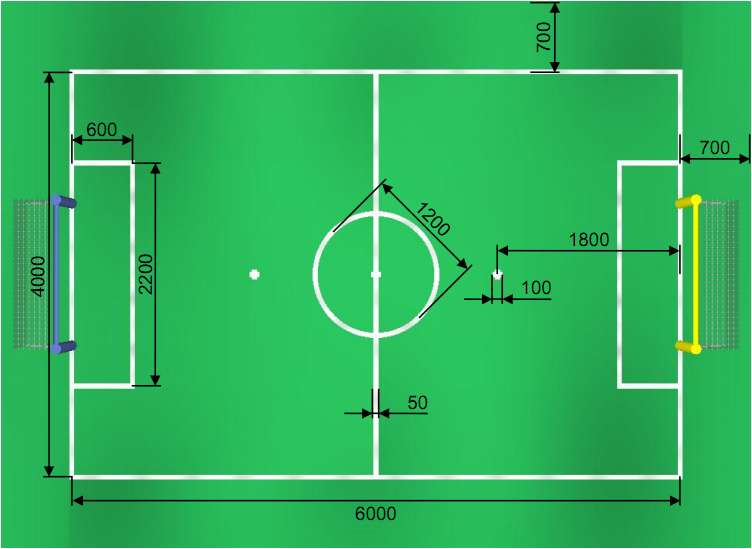
\includegraphics[width=0.5\textwidth]{Pictures/field.png}
\caption{The standard field layout for Robocup SPL 2011 showing the white field-lines.}\label{fig:field}
\end{figure}

Field lines (Figure \ref{fig:field}), on the other hand, are present all around the field in a variety of shapes and formations, often in locations that are very convenient to look at. Even though not unique, these features can provide accurate information about a robot's location. Observation of field-line features are used to provide a likelihood function of the observation given the state of the robot that is passed to a multi-modal Kalman filter \cite{claridge}\footnote{A discussion of the filter is beyond the scope of this paper}. 

The aim of this paper is to describe the development of an efficient algorithm to identify the field-lines using vision and to build more complex features from them to help localise the robot. In particular, the goal is to develop a system with the following characteristics:

{\bf Accuracy:} It should accurately report distances, headings and orientations of all identified field lines in compliance with a vision-localisation interface. False-positive identifications should be minimised. 

{\bf Speed:} It should be fast enough that the entire perception pipeline can run on a 500 MHz GEODE processor in less than 30 milliseconds as the camera frame-rate is 30 fps. The perception cycle needs to leave computing resource available for all the other functions to run the robot's behaviours in the most reactive way for competitive play. 

{\bf Robustness:} The system should be resistant to noise due to the movement of the camera during bipedal locomotion of the robot and the changing occlusion of field-lines by the other seven robots and several referees.

{\bf Modularity:} It should be modular to allow re-use of common components and separate simultaneous vision development by other members of the team.

In the Background Section we review related work by other researchers in this area. We describe our approach in the Methodology Section detailing the RANSAC algorithm for detecting basic lines and circles from which more complex features are constructed. We show the results with images taken from Nao robots used in the SPL, finally providing an evaluation and pointers to future work. 

\section{Background}

We review several approaches taken by others in the detection of filed-line points, and simple and more complex features. 

\subsection{Generating Candidate Points} 
The first step in many feature detection algorithms used in vision is to generate a list of candidate points or regions.

\citeauthor{rUNSWift2010} \shortcite{rUNSWift2010} use colour as the basis for generating candidate field-line points . The algorithm involves scanning vertically down an image looking for changes in colour from green to white or white to green and marking each of these points as field line points. This simplistic approach means that this section of the algorithm runs quickly, as there is little to no processing required on each pixel from the colour saliency. It is heavily integrated into the rest of the vision system. Only using a vertical scan means that any field-lines that are close to vertical in the image are difficult to detect because they only appear in a very small number of scans and thus only generate a small number of candidate points.

\citeauthor{BHumanCodeRelease2010} \shortcite{BHumanCodeRelease2010} used a similar approach of scanning vertically through a colour classified image. They build candidate regions as opposed to identifying candidate points. Their algorithm uses the vertical scan to identify small regions and then group adjacent regions together to form larger ones. The vertical nature of their scan means that they too have to deal with the difficulty of detecting  vertical lines, especially since such lines appear as only a small number of regions.

\citeauthor{NaoDevils2010} \shortcite{NaoDevils2010} also approach scanning using a colour classified image. They use radial scan-lines instead of vertical scan-lines. Radial scan-lines originate at the centre of the robot and pan outwards like the radii of a circle, meaning that they are almost vertical, but slightly tilted. This approach also has to deal with the problem of near-vertical lines not being detected by the scans.

A factor in each of the above approaches is that they depend on accurate colour calibrations. While this problem can be avoided by having a good colour classification table, it can sometimes be difficult to imitate the exact lighting conditions of a game situation as lighting easily varies. \citeauthor{HTWK2011} \shortcite{HTWK2011} have a unique approach for their vision algorithms in that they use colour classification minimally. They instead rely heavily on edge information to generate candidate field-line points which means that they are not nearly as vulnerable to changes in lighting conditions and do not need to spend time setting up colour tables for each new environment.

Present methods for detecting candidate field-line points rarely work in all cases. Most approaches require the implementation of extra functionality to accurately identify points on vertical field-lines and many are also heavily reliant on colour tables.

\subsection{Detecting Simple Shapes}

Once a list of candidate points has been generated, the next step is to try and form lines and circles using these points. 

\citeauthor{BHumanCodeRelease2010} \shortcite{BHumanCodeRelease2010} use a clustering based algorithm to group small segments they generate into long field-lines. Their method includes representing each segment in Hesse normal form and grouping segments that have similar distance and direction values into longer lines. The problem with the clustering algorithm was that it is modified to run in $O(n^2)$ time worst case and thus is not guaranteed to find optimal clusters. The left-over line segments are used to detect a circle by calculating the perpendicular bisector of each segment, intersecting it with the perpendicular bisector of each adjacent segment, and clustering them together using the original clustering algorithm. The issue is that optimal clusters are sacrificed to ensure efficient run time, meaning that many sanity checks are required to ensure accurate results.

\citeauthor{UPenn2010} \shortcite{UPenn2010} took a unique approach and optimised the otherwise too Hough transform \cite{HoughTransform} for use in line detection. Unfortunately they only considered one line or circle per image (possibly due to time constraints) so are not able to demonstrate its full power at competition.

Thus it is clear that there is room for several improvements in the observation of field-lines utilising efficient and accurate line and circle detection algorithms.

\subsection{Compound Field Features}
The SPL uses a standard field format for competition. The 2011 the field layout is shown in Figure \ref{fig:field}. It looks similar to a normal soccer field with several identifiable field-line features such as:

\begin{description}
\item[Lines]: There are 11 straight lines spread around the field.
\item[Corners]: Two field lines intersect in 8 places on the field to form a corner.
\item[T-Intersection]: Two field lines intersect in 6 places on the field to form a T-intersection.
\item[Centre Circle]: The circle in the middle of the field is the only circle and has a line intersecting it.
\item[Penalty Spot]: There are two penalty spots on the field, one in each half.
\item[Goal Box]: The goal area is surrounded by a box shape, which can be broken down into two pairs of parallel lines.
\end{description}

All of these features have useful information to pass through to localisation and can be vital in keeping the robot localised without having to look around for goal-posts. Few teams in the SPL can detect all the listed features. 

The \citeauthor{UPenn2010} \shortcite{UPenn2010} is only able to detect a single line per frame. Whilst this is still very useful for maintaining a good localisation, it is not sufficient if the robot is lost.

\citeauthor{uTAustin2010} \shortcite{uTAustin2010} is able to utilise lines and circles in each frame. The use of multiple lines instead of just a single line gives them greater precision when calculating a position from the lines. This and the centre circle also allows improved ``kidnapped" robot detection as multiple shapes can be matched to sections on the field.

\citeauthor{Edinferno2010} \shortcite{Edinferno2010} use an interesting combination of features detecting the centre circle and the penalty spot. This gives them a fairly good distribution of landmarks across the field. However, they are missing significant information by not considering straight lines, which are the most common feature on the field.

\citeauthor{NaoDevils2010} \shortcite{NaoDevils2010} detect lines, corners, T-intersections, unidentified intersections and the centre circle. The corners and T-intersections are extremely useful for both fine-tuning a well localised robot's position and to solve the kidnapped robot problem. The unidentified intersection utilises every piece of information in the frame, even if the frame doesn't allow for detection of exactly which intersection had been seen. They also utilise the centre circle by using its intersecting line. The combination of the line and circle generates just two symmetrical hypotheses and makes it a useful update both for a well localised robot and for a kidnapped robot.

\citeauthor{rUNSWift2010} \shortcite{rUNSWift2010} do not detect shapes and therefore do not have the ability for field-lines to be used to localise a lost robot. They are only able to do a local update to tune a localised robot's position using a set of points. This approach does not work  if robot is not close to where it believes it is. 

Field-line detection is an area that the Standard Platform League can improve. In this paper we describe research and development of a system to fill this gap.

\section{Methodology}

We will first introduce RANSAC and other preliminary concepts before describing our approach to field-line detection and the formation of more complex features. 

\subsection{RANSAC for Image Analysis}
Random Sample Consensus (RANSAC) \cite{Fischler:1981:RSC:358669.358692} is an iterative approach to estimate parameters of a model from a set of data that contains outliers. The algorithm works on the assumption that the data consists of inliers, whose distribution can be explained by some set of parameters, and outliers that do not fit the model. An example is fitting a line to a set of points in 2D space. RANSAC is demonstrated in Figure \ref{fig:ransac}.

\begin{figure}[H]
\centering
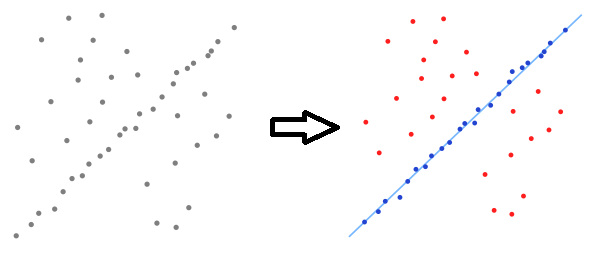
\includegraphics[width=0.5\textwidth]{Pictures/ransac.png}
\caption{A data set with many outliers having a line fitted by the RANSAC algorithm. Notice that the line best fits the inliers instead of the entire data set. (diagram from Wikipedia)}
\label{fig:ransac}
\end{figure}

Starting with a set of points in 2D space, the RANSAC algorithm picks two points and generates a line between them. It then calculates which points from the original data set are now considered part of this line based on their distance to the line. Each of these `inliers' are considered part of the line and are used to generate a measure of variance (an error) of the line's fit to the dataset. This is repeated for a predetermined number of runs, during which time it is hoped that two points from the correct subset of data are chosen. The algorithm works well because the line fits the set of inliers optimally instead of trying to fit the entire dataset optimally.

While this is a fairly specific example, the above methodology can be used on a variety of shapes (including circles) as well as applications not relevant to computer vision algorithms. It is a useful algorithm because of a good speed versus accuracy trade-off where only a very small amount of accuracy is traded away (especially if the data set contains lots of inliers) for a very large increase in speed.


\subsection{Edge Saliency}
Our \emph{edge saliency} image is a down-sampled $80 \times 60$ image from the original $640 \times 480$ image containing two values for each pixel. The first value represents the change across the horizontal direction ($dx$) and the second represents the change across the vertical direction ($dy$). It is generated by taking a grey scale version of the original $640 \times 480$ raw camera image, applying a Gaussian smoothing operation and calculating the $dx$ and $dy$ using a formula that models local change \cite{chatfield}. These two values allow us to determine both a magnitude and a direction for each of the pixels\footnote{the equation avoids an expensive square-root operation}:

\begin{eqnarray}
Magnitude^2 &=& dx^2 + dy^2\\
Direction &=& \arctan(\frac{dy}{dx})
\end{eqnarray}


\subsection{Image Plane vs Ground Plane}
Points that are in the \emph{image plane} are represented in terms of their $x$ and $y$ coordinates in the saliency image. This means that a point in the very bottom right corner of the image is at $(79, 59)$ whilst a point in the very top left of the image is at $(0,0)$. In contrast to this, the \emph{ground plane} represents the 2D plane of the physical floor space around the robot. For example, in the robot-relative co-ordiante system, the point $(0,0)$ in the ground plane is directly underneath the centre of the robot, whilst the point $(1000, 0)$ is 1000 millimeters in front of the robot. Pixels in the image have a direct mapping to points on the field and this is calculated through the kinematic chain developed by \citeauthor{rUNSWift2010} \shortcite{rUNSWift2010}. 

\subsection{Generating Candidate Points}
The first step in the process of detecting field features is to identify candidate points that may make up part of each feature. This approach utilises edge data to find candidate points. The idea is to scan vertically and horizontally through the image, looking for a pair of edges that fulfil the criteria of possible field line points.

The algorithm performs a vertical scan in a downwards fashion through the edge saliency image. If the edge of the field is detected, we only scan below that, if not we scan the entire image. For each pixel we consider how strong the magnitude of edge is at that point. If the edge is weak, we skip it and move on. If it is a strong edge, we consider which side of the field line it might represent (since it could be a green - white edge or a white - green edge). It is reasonable to assume that the first edge found should be a green - white edge. Once this first edge is found, we store its magnitude and direction for use later and move to the next point.

Upon reaching the next strong edge point, we consider whether it is part of the first edge, part of the matching white-green edge on the other side of the field line, or just a random bit of noise. We examining the direction of the edge. If the edge is a similar direction to the first edge, it is probably part of that top edge and has just spanned more than 1 pixel in width. In this case, we compare the magnitudes of this point with the currently saved top edge point and only keep the strongest pixel one.

If the next point's direction is approximately opposite in direction to the first point, then it is considered as part of the bottom side of the field-line. Similar to the top side, there can be multiple points detected as part of the bottom edge (assuming they all have a similar direction), but only the point with the highest magnitude is stored.

There is also a possibility that the second point fits neither of the above two categories, in which case it is assumed that the first point is actually the top of a field line and thus is considered noise. Since we cannot tell if the second point is valid or not, we set it to be the new first point and continue the search for a second point.

The scan continues downwards until either it reaches the bottom image, or stops hitting strong edges. If it stops hitting strong edges then we have finished scanning the field-line. If we have detected both a top edge and a matching bottom edge we calculate the midpoint of the two to give us the centre of the field-line. To confirm the hypothesis we perform a variety of sanity checks to ensure that we have identified a candidate point. They are:

\begin{itemize}
\item The top and bottom points should be opposite in direction (already tested implicitly by the algorithm)
\item	The top and bottom points should be roughly 50mm apart in the ground plane
%\item	The midpoint should not be too far away [what does this mean?]
\item	The midpoint should be white in the Colour Saliency
\end{itemize}

If the sanity checks are passed, we consider the point to be a candidate for a field-line point and save it in a list along with information about the point. We store a $dx$ and $dy$ value for the midpoint, which is calculated as the average of the top and bottom point's $dx$ and $dy$, the coordinates of the pixel in the image plane, and the coordinates of the pixel in the ground plane.

Once all the columns have been scanned, the next step is to determine if any horizontal scans are necessary. We do not want to scan over areas that have already been scanned because it wastes computing resources and generates duplicates in our list of points. Thus the horizontal scan is only performed if the row has some section below the field edge and if the row doesn't already have some field line points in it.

If we decide to perform a horizontal scan, the algorithm used is the same as the vertical scan, except that the top and bottom of the line now represent the left and the right sides of the line. The procedure is otherwise identical. 

\subsection{Detecting Lines and Circles}
The first step in detecting simple shapes is to convert all the points detected previously into the ground plane where lines and curves are easier to distinguish. 

We then run a combined RANSAC line and circle function (Algorithm \ref{alg:ransac})  where for each two points picked at random, both a line and circle are generated between them. 

The algorithm  runs as follows: to begin we pick two points at random from the list of candidates generated above. The line defined by these two points is then calculated and the distance to each point is computed. If a point lies within the minimum distance, it is considered on the line and thus is marked and added to the variance (error function). Once all the distances have been calculated, the variance is finalised, compared with the current best and if better is saved instead. A circle of radius 600mm (see Figure \ref{fig:field}) is calculated through those points (the direction is chosen at random) and the distance from each point to the circle calculated. Similar to the line, all the points within the minimum distance are marked and added to the variance. The variance of the circle is compared against the best and saved if better. This entire process is repeated a set number of times.


\begin{algorithm} [h] 
\caption{RANSAC Line and Circle}
\begin{algorithmic} \label{alg:ransac}

\STATE $i \leftarrow 0$
\STATE $radius \leftarrow 600$
\STATE $bestLineVariance \leftarrow max$
\STATE $bestCircleVariance \leftarrow max$
\WHILE{$i < k$}
	\STATE $p1 = points[rand\%size]$
	\STATE $p2 = points[rand\%size]$
	
	\STATE $line = line(p1, p2)$
		
	\FORALL{$p \in points$}
		\STATE $distance = \frac{|line.t1*p.x + line.t2*p.y + line.t3|}{\sqrt{line.t1^2 + line.t2^2}}$
		\IF{$distance < e$}
			\STATE $variance \leftarrow variance + distance$
			\STATE $numPoints \leftarrow numPoints + 1$
		\ENDIF
	\ENDFOR
	\STATE $variance \leftarrow variance * 0.2 - numPoints$
	\IF{$variance < bestVariance$}
		\STATE $bestVariance = variance$
	\ENDIF
	
	\STATE $circle = circle(p1, p2, radius)$
	\FORALL{$p \in points$}
		\STATE $c \leftarrow circle.centre$
		\STATE $distance = \sqrt{(c.x - p.x)^2 + (c.y - p.y)^2} - radius$
		\IF{$distance < e$}
			\STATE $variance \leftarrow variance + distance^2$
			\STATE $numPoints \leftarrow numPoints + 1$
		\ENDIF
	\ENDFOR
	\STATE $variance \leftarrow variance * 0.2 - numPoints$
	\IF{$variance < bestVariance$}
		\STATE $bestVariance = variance$
	\ENDIF
	
	\STATE $i \leftarrow i + 1$
\ENDWHILE

\end{algorithmic}
\end{algorithm}


This innovative approach eliminates a problem where a RANSAC line function would pick up points better suited to the circle, whilst a RANSAC circle function would pick up points better suited to a line. The idea is to run the two algorithms in parallel, compare the final results and take the better of the two.

One of the challenges with this approach is that it requires a metric for comparing circles and lines to each other. Whilst the variance of one line is comparable to another, it isn't necessarily comparable to a circle's variance. In the end a fairly simple variance calculation involving the sum of the distances to each point and the number of points, with a slight bias towards lines, was enough to accurately compare the two shapes and ensure that even a small segment of either shape was accurately identified as the correct shape.

\subsection{Detecting Field Features}
Field-line segments are highly aliased. We would like to form highly discriminative compound features to concentrate the observation likelihood distribution. In this regard we are able to detect corners, T-intersections, pairs of parallel lines, the centre circle and halfway line, together with the simple circles and lines.

\subsubsection{Intersections - Corners and T's}
The process for finding intersections involves scanning through the list of lines detected and seeing if each one intersects any of the other lines. Whilst this approach is technically $O(n^2)$ there are so few lines detected in one frame that the time complexity isn't a factor, especially since the calculations are quite efficient. For an optimised method to find the intersection between two lines we use two matrices and perform an LU decomposition. If the equations have a solution then the lines intersect and we know the point of intersection.

Sanity checks are applied at this point of the algorithm. For the point of intersection to be considered for further examination it has to occur not only within the image, but also at least 8 pixels from the edge. The two lines that intersect need to be approximately perpendicular, otherwise they cannot be a corner or a T-intersection.

If the sanity checks pass, the next step is to identify the type of intersection. Since the endpoints of each line are not known it is difficult to determine if the intersection is a corner or a T. The method used to differentiate between the two relies on the fact that in a corner all the points belonging to one line should lie on one side of the other line, and vice versa. For a T intersection one line should have all its points on one side of the other, whilst the other line should have points on both sides of the first line. With this in mind, the algorithm for determining if we have a T-intersection involves calculating the distance to each point on the other line and incrementing either the negative or positive tally depending on the sign of the distance. If we get enough points on either side of a line, then the function returns true.

This algorithm is run twice, one with the points from line2 against line1, then with the points from line1 against line2. Afterwards, if both times it returns false then it is probably a corner, if only one returns true then it is a T-intersection and if both return true it has detected some sort of X-intersection and discarded. Once the intersection type has been confirmed and all the sanity checks are passed, the point of intersection is transformed into the ground plane and stored.

The next step is to calculate the distance, heading and orientation of the feature. Calculating the distance and heading to each feature is a simple matter of calculating the distance and angle  between the robot and the feature in the ground plane. Calculating orientation involves basic geometry and uses a combination of the heading and the feature's rotation in space. If the intersection is $(X,Y)$, the formulas are as follows:

\begin{eqnarray}
Distance &=& \sqrt{X^2 + Y^2}\\
Heading &=& \arctan{(\frac{Y}{X})}\\
Orientation &=& \left\{ \begin{array}{rl}
heading - rotation + 180\\ \mbox{ if $rotation > 0$} \\
heading - rotation - 180\\ \mbox{ otherwise}
\end{array} \right.
\end{eqnarray}

The rotation of a feature is defined as the angle between the `primary line' of the feature and the line from the robot to the feature. For a corner the primary line is defined as being the line that bisects the corner, whilst for a T-intersection the primary line is defined as being the upright line in a T. Figure \ref{fig:corners} shows the $(x, y, orientation)$ of four corner types.

\begin{figure}[H]
\centering
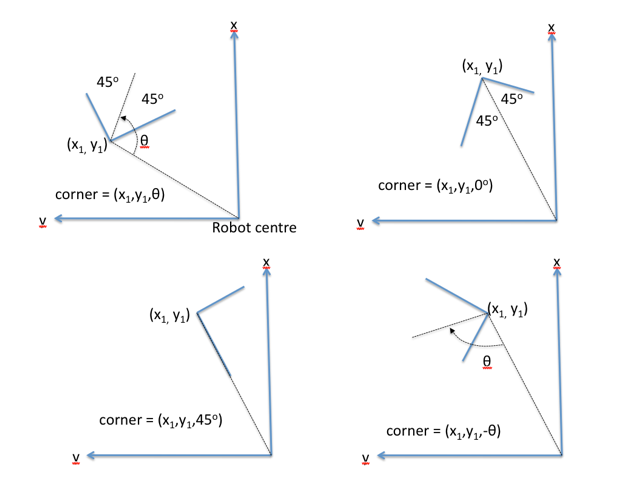
\includegraphics[width=0.5\textwidth]{Pictures/orientation.png}
\caption{Four examples of corner orientation orientations.}
\label{fig:corners}
\end{figure}

\subsubsection{Centre Circle}
Most of the work for the centre circle detection has already been done by detecting the circle in the RANSAC section. It calculates the location of the centre of the circle in the ground plane, and its distance and heading can be calculated as above. The orientation of a circle is undefined, but if we detect the half-way field-line as well, we can give the combination an orientation. In this case we define the orientation to be the angle between the line to the centre and the half-way line. The formula is as follows:

\begin{eqnarray}
& Orientation = \nonumber \\ 
& robotToCentreDirection - centreLineDirection
\end{eqnarray}

%The method for finding the direction of the two lines used for the orientation is just a simple vector direction calculation similar to the following.

%\begin{equation}
%Direction = \arctan{(\frac{vectorY}{vectorX})}
%\end{equation}

\subsubsection{Parallel Pair}
If any straight lines form perpendicular intersections, they are removed from the list of lines by the time this point in the algorithm is reached. Thus the only lines passed to this function must not intersect at right angles. With this in mind, the first thing to look for is lines that are roughly parallel. This is a simple calculation where we look at the angle of the two lines relative to the robot and see if they are within a threshold value. If they are, we also need to check how far apart they are from each other. Since this feature is representative of the goal line and the edge of the goal box, the lines should be approximately the same distance apart as those two lines are on the field - ie 600mm. 

If both of the above sanity checks are passed, we can be satisfied that we have a parallel pair and the information is stored to be passed to localisation. The information that we do pass on for this feature includes the data for the closest line as well as the perpendicular distance and heading to the first line. They are calculated as follows:

\begin{eqnarray}
Perpendicular Distance = \frac{|line.t3|}{\sqrt{line.t1^2 + line.t2^2}}\\
Heading = \arctan{(\frac{-line.t1 * line.t3}{(line.t2 * line.t3})}
\end{eqnarray}


\section{Results}
We conducted several experiments to test the operation of our RANSAC field-line detector. 

\subsection{Experiment 1 - Centre Circle}
The first experiment involves placing a robot near the centre circle looking towards the area where the circle intersects the halfway line (Figure \ref{fig:exp1}). We've added some extra display information to show the top and bottom edge-points of the field-lines to illustrate how the pair-matching works. The top/left edges are represented by the red pixels, the bottom/right edges are represented by the blue pixels, and the midpoints are represented by white pixels. When the top and bottom edges are adjacent the midpoint has the same pixel location as one of the edges, and thus is drawn over in some occasions. Here we can see that the algorithm has picked up a good number of points both on the circle and on the line intersecting it.

\begin{figure}
\centering
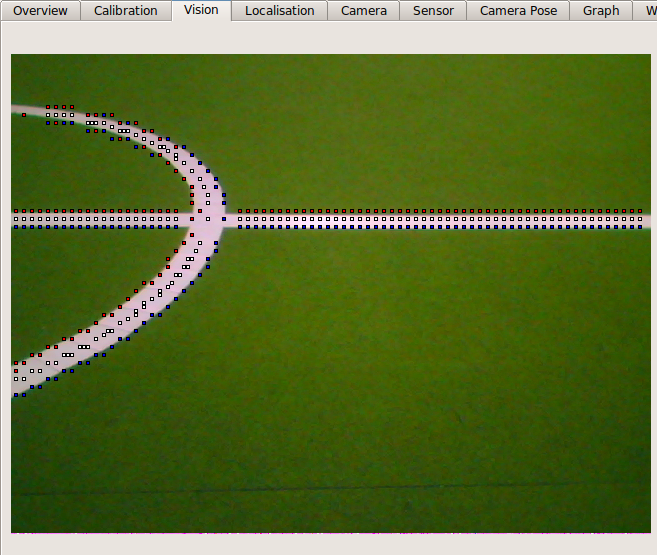
\includegraphics[width=0.4\textwidth]{Pictures/candidateCircle.png}
\caption{Candidate point selection algorithm shown with red representing the top edges, white the midpoints and blue the bottom edges}
\label{fig:exp1}
\end{figure}

\subsection{Experiment 2 - Corner}
The second experiment involves placing a robot looking at one of the corners about 1m away. As can be seen from the overview tab in Figure \ref{fig:exp2} where the yellow circle is the robot, we used one of the goal box corners. In this scenario the robot detects both sides of the box, intersects them and matches the intersection to a corner. In the field view the tiny blue strip represents candidate points, the red lines represent the detected lines, while the black L shape represents the corner that has been detected.

\begin{figure}[h]
\centering
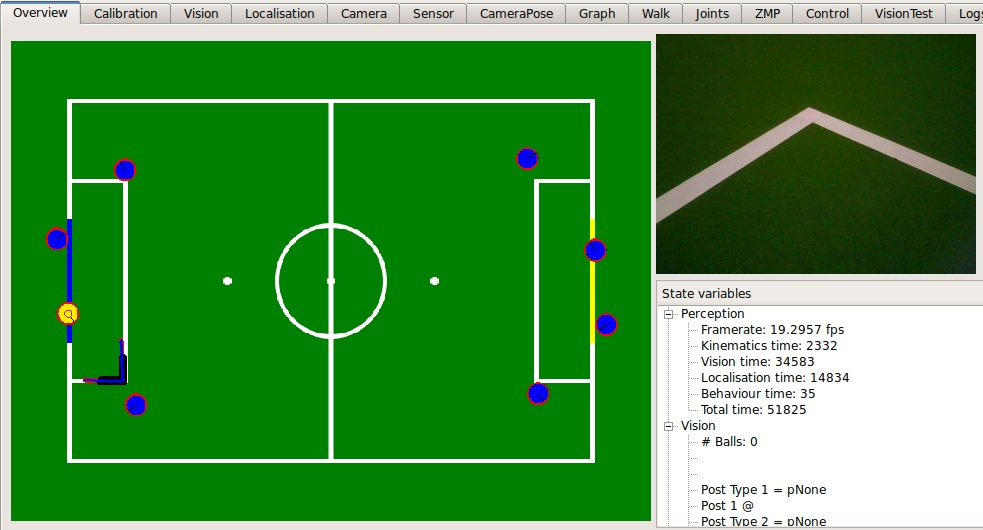
\includegraphics[width=0.5\textwidth]{Pictures/cornerIntersection.jpg}
\caption{Corner detection and the corresponding modes generated by localisation around the field}
\label{fig:exp2}
\end{figure}

\subsection{Experiment 3 - T-Intersection}
The third experiment involves placing a robot on the halfway line looking at the T-intersection formed by the halfway line meeting the sideline. As shown in Figure \ref{fig:exp3} both the sideline and halfway are detected and a T-intersection is formed between them. Notice how localisation generates a total of 6 modes, each one facing a different T-intersection around the field. In this case the multi-modal Kalman filter, due to the lack of information in the image, has choosen the incorrect mode as the primary one (yellow).

\begin{figure}[h]
\centering
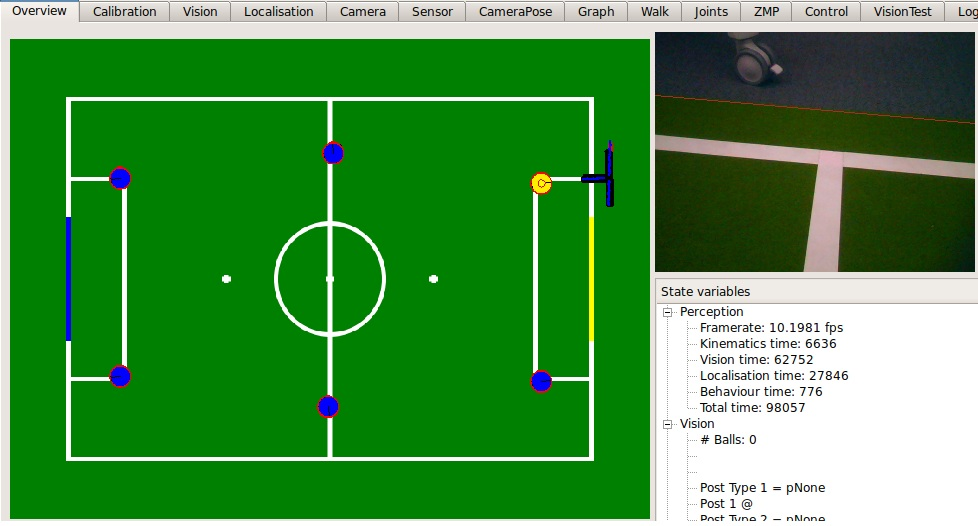
\includegraphics[width=0.5\textwidth]{Pictures/tIntersection.jpg}
\caption{T-Intersection detection and the corresponding modes generated by localisation around the field}
\label{fig:exp3}
\end{figure}

\subsection{Experiment 4 - Maximum Distances}
The fourth experiment involves placing the robot near the goal line and the edge of the goal-box, as shown by the yellow circle in Figure \ref{fig:exp4}. In this scenario the goal line is approximately 1.5m away and very few candidate points are generated on it. The other two lines on the goal box both generate a fair set of candidate points via both the horizontal and vertical scans.

\begin{figure}[h]
\centering
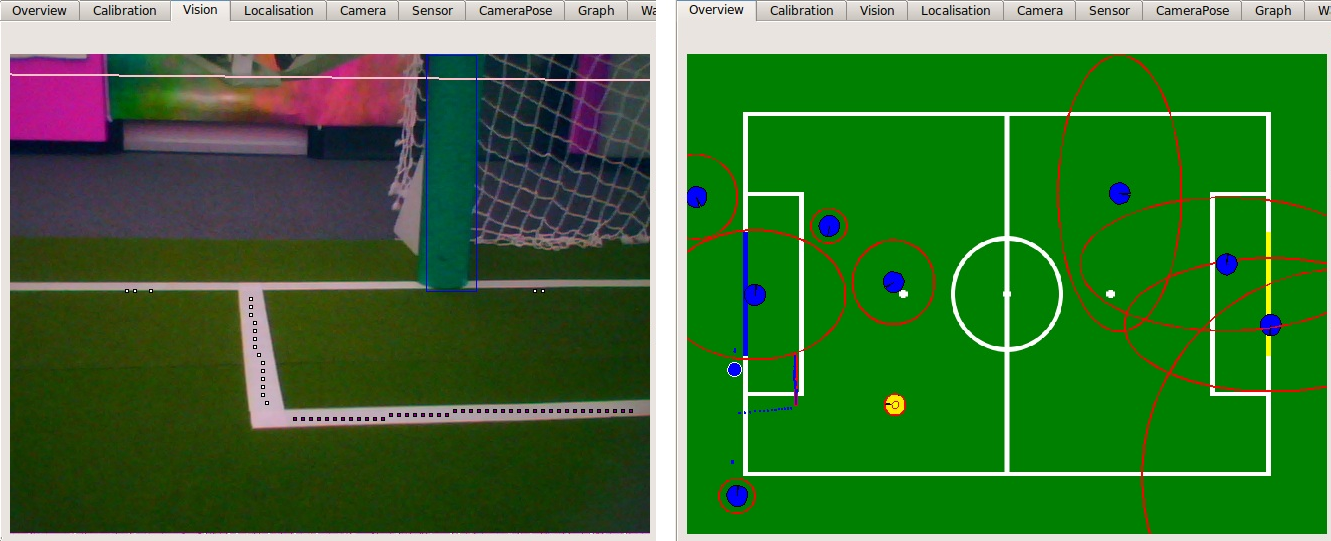
\includegraphics[width=0.5\textwidth]{Pictures/candidateT2.png}
\caption{Candidate point selection algorithm struggles to identify the goal line at a distance of around 1.5m}
\label{fig:exp4}
\end{figure}


\subsection{Experiment 5 - Double Line}
The fifth experiment hightlights more issues caused by the low resolution. It involves placing a robot near the limit at which it can detect a line, so approximately 1.4m from the goal line. As can be seen from the vision tab in Figure \ref{fig:exp5}, the points on the goal line are two different colours, indicating that they have been detected as 2 separate lines, despite actually all being part of the goal line.

\begin{figure}[H]
\centering
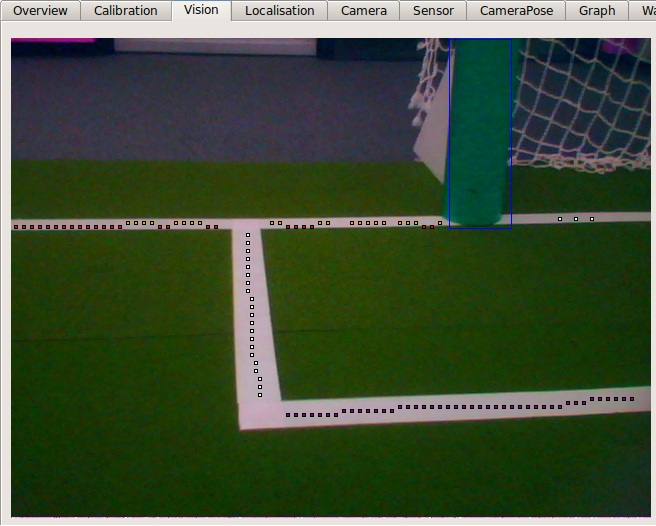
\includegraphics[width=0.5\textwidth]{Pictures/doubleLine.jpg}
\caption{The red points belong to one line whilst the orange points belong to a separate one}
\label{fig:exp5}
\end{figure}


\subsection{Experiment 6 - Centre Circle and Halfway Line}
The sixth experiment involves placing a robot about a metre from the halfway line, looking towards the centre circle (Figure \ref{fig:exp6}). From this position, the centre circle and the halfway line are both detected, as shown by the red circle and red line in the field view. Notice this time how there are only 2 modes generated by localisation.  This is because this frame can only be replicated at a total of 2 positions on the field, making it an extremely useful observation.

\begin{figure}[H]
\centering
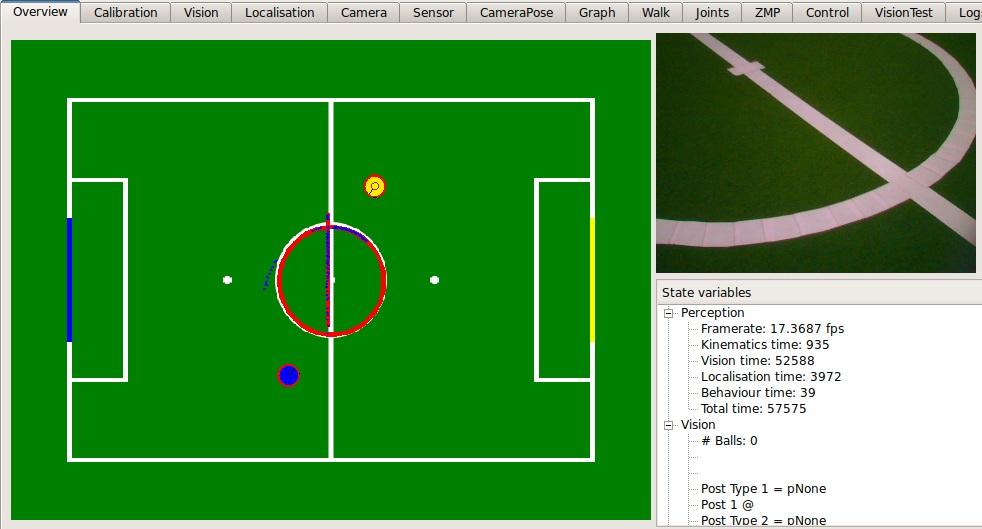
\includegraphics[width=0.5\textwidth]{Pictures/circleHalfway.jpg}
\caption{Centre circle and halfway line detection and the corresponding modes generated by localisation around the field}
\label{fig:exp6}
\end{figure}


\subsection{Experiment 7 - Goal Box}
The seventh experiment involves placing a robot between 1 and 1.5 metres from the goal line, near the corner of the goal box. At approximately 1.3m from the goal box, the shorter vertical segment does not receive enough points to fulfil the minimum number of points and is not classified as a line. This is demonstrated in Figure \ref{fig:exp7} where it can be seen that there are many blue points in the area, but no red line over the top. Notice also that the two parallel lines are black, indicating that they are identified as a parallel pair.

\begin{figure}[H]
\centering
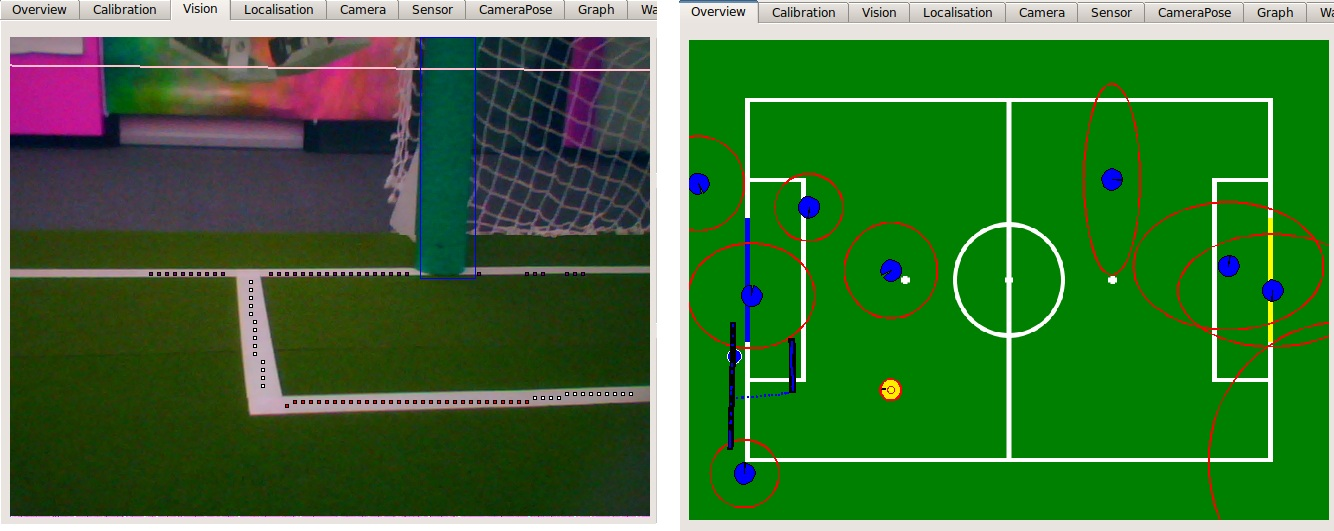
\includegraphics[width=0.5\textwidth]{Pictures/goalBox.jpg}
\caption{Line detection is unable to match a line to the short goal box segment}
\label{fig:exp7}
\end{figure}



\section{Evaluation}
%TODO fix experiment numbers
From the above results it is clear that field line features can be accurately detected up to a distance of 1.5 metres. Experiment TODO shows how generating both a line and a circle for each pair of points and considering their variances against each other gives an accurate method for differentiating between lines and circles in an image. It also shows just how useful detecting both the centre circle and halfway line in one image really is.

Experiments 2 and 3 show the full power of combining straight lines into features found around the field, like corners and T-intersections. It shows the usefulness of these updates not only for a robot that has a rough idea of where it is, but also one that has become lost and has no idea where it is.

For lines that appear further than 1.5 metres there are few to no points detected. This deterioration is primarily due to inaccuracies in distance measurements caused by the low resolution of the saliency image. At a distance of around 1.5 metres, vertically adjacent pixels are around 50mm apart. This means that the top and bottom pixels need to be literally adjacent to be approximately 50mm apart. To compensate for these inaccuracies, the sanity check for the top and bottom pixels being approximately 50mm apart actually allows them to be up to 200mm apart before rejecting them. Unfortunately in the edge saliency, field lines at a distance of about 1.5m can have the top and bottom edges being 4-5 pixels apart, which translate into 250mm in the ground plane. Thus this sanity check often eliminates far away field-line points simply because of inaccurate distance measurements. Despite this, the sanity check is very useful in eliminating false positive inside robots because they are much wider than field lines.

The low resolution also proves problematic in Experiment TODO where despite being only 1 pixel higher, the points on the top line are considered 50mm away from the points below once they are projected into the ground plane. Since the distance for points to be part of a line or circle is only 15mm, these points are much too far apart to be considered one line when in the image they clearly are.

Experiment TODO shows how the goal box line isn't always identified despite comprising many candidate points. The reason for this is the high value of the RANSAC $n$ variable, which determines how many points are required to form a line or circle. This value was set high to ensure that noise like robot points (in particular their arms) does not cause any false positive lines. As a result this line is often missed, which led to the development of the parallel pair feature. By detecting both the lines and identifying them as parallel and 600mm apart, the robot can be certain that the lines belong to one of the goal boxes and can therefore provide an accurate X-axis update as well as a heading update. This allows the information detected to be utilised despite the potential shortcomings of the line detection.


\section{Future Work}
\subsection{Detecting the Penalty Spot}
Penalty spot detection was not implemented primarily because they cannot be easily constructed from the line and circle models. The candidate points detected are too few for reliable classification as a line or a circle. They are discarded by the RANSAC algorithm as outliers. Penalty spot detection would be difficult to implement at a distance of more than a metre, due to the low number of candidate points it would generate. It would be quite difficult to differentiate the penalty spot from noise or even a robot section with so few points.

At a closer distance however, the penalty spot generates a fair number of points which actually resemble a cross shape. These points could be grouped together using a simple clustering algorithm or blog detection algorithm but it might take some work to not generate false positives inside robots. There might even be enough information at close range to implement a cross based version of RANSAC to match the shape of the points to a cross.

\subsection{Utilising Foveas}
Another potential avenue of improvement would be to utilise the foveas developed by Chatfield \shortcite{chatfield} to detect far away balls to also detect far away field-lines. These foveas allow you to zoom in on a particular section of each image for high resolution analysis and would help remove many of the errors generated by the low resolution of the saliency image. This would allow field lines to be detected at far greater distances and could even improve the accuracy of closer field features detected.

This would also come with its own set of challenges though, as some sort of algorithm would need to be developed to decide which area of the image is worth investigating at higher resolution. The way the vision system is currently set up, if a good algorithm for picking the area of the original image to focus on was developed, the current field-line detection code could be run using the high resolution fovea instead of the low resolution image with minimal changes.

\subsection{Unidentified Intersections}
One shortcoming in the current system is that we do not report an intersection between perpendicular lines unless it is clearly in the visual frame and we can identify exactly the type of the intersection it is. While this does still occur fairly often, there are also a large number of times when the point of  intersection is just outside the frame, or is close to the edge so it is hard to detect precisely what type of intersection it is. Rather than just throw this information away, it could be instead labelled as an unidentified intersection and still passed on to localisation.

This change could be implemented easily with a few lines of code in field-line detection to instead save intersections sanity checked out because they do not land in the middle of the image. The problem with adding this is that the localisation module would require a fair bit of work to also accommodate the changes.

\section{Conclusion}
This paper has presented a creative and efficient methodology for detecting field-line features using RANSAC. At each stage of the process we have been able to achieve accurate and reasonably fast results which, in combintation, form a pipeline to detect a variety of field-line features across a soccer field.

\section{ACKNOWLEDGMENTS}

The authors gratefully acknowledge the support of the School of Computer Science and Engineering, other members of the 2011 rUNSWift team, and associated staff and students in the school's robotic laboratory.

\bibliographystyle{named}
\bibliography{references}

\end{document}

